\documentclass[english]{article}\usepackage[]{graphicx}\usepackage[]{color}
%% maxwidth is the original width if it is less than linewidth
%% otherwise use linewidth (to make sure the graphics do not exceed the margin)
\makeatletter
\def\maxwidth{ %
  \ifdim\Gin@nat@width>\linewidth
    \linewidth
  \else
    \Gin@nat@width
  \fi
}
\makeatother

\definecolor{fgcolor}{rgb}{0.345, 0.345, 0.345}
\newcommand{\hlnum}[1]{\textcolor[rgb]{0.686,0.059,0.569}{#1}}%
\newcommand{\hlstr}[1]{\textcolor[rgb]{0.192,0.494,0.8}{#1}}%
\newcommand{\hlcom}[1]{\textcolor[rgb]{0.678,0.584,0.686}{\textit{#1}}}%
\newcommand{\hlopt}[1]{\textcolor[rgb]{0,0,0}{#1}}%
\newcommand{\hlstd}[1]{\textcolor[rgb]{0.345,0.345,0.345}{#1}}%
\newcommand{\hlkwa}[1]{\textcolor[rgb]{0.161,0.373,0.58}{\textbf{#1}}}%
\newcommand{\hlkwb}[1]{\textcolor[rgb]{0.69,0.353,0.396}{#1}}%
\newcommand{\hlkwc}[1]{\textcolor[rgb]{0.333,0.667,0.333}{#1}}%
\newcommand{\hlkwd}[1]{\textcolor[rgb]{0.737,0.353,0.396}{\textbf{#1}}}%

\usepackage{framed}
\makeatletter
\newenvironment{kframe}{%
 \def\at@end@of@kframe{}%
 \ifinner\ifhmode%
  \def\at@end@of@kframe{\end{minipage}}%
  \begin{minipage}{\columnwidth}%
 \fi\fi%
 \def\FrameCommand##1{\hskip\@totalleftmargin \hskip-\fboxsep
 \colorbox{shadecolor}{##1}\hskip-\fboxsep
     % There is no \\@totalrightmargin, so:
     \hskip-\linewidth \hskip-\@totalleftmargin \hskip\columnwidth}%
 \MakeFramed {\advance\hsize-\width
   \@totalleftmargin\z@ \linewidth\hsize
   \@setminipage}}%
 {\par\unskip\endMakeFramed%
 \at@end@of@kframe}
\makeatother

\definecolor{shadecolor}{rgb}{.97, .97, .97}
\definecolor{messagecolor}{rgb}{0, 0, 0}
\definecolor{warningcolor}{rgb}{1, 0, 1}
\definecolor{errorcolor}{rgb}{1, 0, 0}
\newenvironment{knitrout}{}{} % an empty environment to be redefined in TeX

\usepackage{alltt}
\usepackage[T1]{fontenc}
\usepackage[latin9]{inputenc}
\usepackage[margin=3cm]{geometry}
\geometry{verbose,tmargin=3cm,bmargin=3cm,lmargin=2.5cm,rmargin=2.5cm}
\setcounter{secnumdepth}{0}
\setcounter{tocdepth}{0}
\usepackage{url, indentfirst}
\usepackage{tabularx, booktabs, multirow, array, caption, color, longtable}
\usepackage{graphicx, fancyhdr, babel, xcolor, csquotes}
\usepackage{hyperref, lineno, setspace, pdflscape}
\usepackage[round]{natbib}
\graphicspath{ {C:/Users/jelber2/Dropbox/LSU/Dissertation/Manuscripts/immunome_2014/rnw/} }

\linenumbers
\doublespacing
\renewcommand\linenumberfont{\small\textnormal}

\title{Population genetic inferences using immune gene SNPs mirror patterns inferred by microsatellites}
\date{}
\author{\\
JEAN P. ELBERS$^{1,3}$, RACHEL W. CLOSTIO$^{2}$, SABRINA S. TAYLOR$^{1}$\\\\
$^{1}$School of Renewable Natural Resources, 227 RNR Bldg., Louisiana State University and AgCenter, \\ Baton Rouge, Louisiana, 70803, USA\\
$^{2}$Department of Biology, 300 E. St. Mary Blvd., University of Louisiana at Lafayette, \\ Lafayette, Louisiana, 70503, USA\\
Keywords: microsatellites, target enrichment, sequence capture, \\ next-generation sequencing, immunogenetics, population genomics \\\\
$^{3}$Corresponding author: Fax: 225-578-4227, Email: \underline{jean.elbers@gmail.com}\\\\
Running title: Immune gene SNPs mirror microsatellites\\\\
}
\IfFileExists{upquote.sty}{\usepackage{upquote}}{}
\begin{document}



\maketitle
\pagebreak{}

\section*{Abstract}
Single nucleotide polymorphisms (SNPs) are replacing microsatellites for population genetic analyses, but it is not apparent how many SNPs are needed or how well SNPs correlate with microsatellites. We used data from the gopher tortoise, \textit{Gopherus polyphemus} - a species with small populations, to compare SNPs and microsatellites to estimate population genetic parameters. Specifically, we compared one SNP dataset (16 tortoises from 4 populations sequenced at 17,901 SNPs) to two microsatellite datasets, a full dataset of 101 tortoises and a partial dataset of 16 tortoises previously genotyped at 10 microsatellites. For the full microsatellite dataset, observed heterozygosity, expected heterozygosity, and \textsc{Fst} were correlated between SNPs and microsatellites; however, allelic richness was not. The same was true for the partial microsatellite dataset, except that allelic richness, but not observed heterozygosity, was correlated. The number of clusters estimated by Structure differed for each dataset (SNPs = 2; partial microsatellite = 3; full microsatellite = 4). PCA showed four clusters for all datasets. More than 800 SNPs were needed to correlate with allelic richness, observed heterozygosity, and expected heterozygosity, but only 100 were needed for \textsc{Fst}. The number of SNPs typically obtained from NGS far exceeds the number needed to correlate with microsatellite parameter estimates. Our study illustrates that diversity, \textsc{Fst}, and PCA results from microsatellites can mirror those obtained with SNPs. These results may be generally applicable to small populations, a defining feature of endangered and threatened species, because theory predicts that genetic drift will tend to outweigh selection in small populations.

\section*{Introduction}
Molecular markers vary in their utility and application to population genetic studies, and geneticists use available markers suited to answering questions at hand. Initially, geneticists only had allozymes and used them to infer nucleotide changes underlying differences in protein migration during electrophoresis. Later, variable mitochondrial DNA markers were used because of the availability of conserved primers and the high copy number of mitochondria, but mitochondrial markers mostly provided information on broad-scale genetic patterns \citep{Moritz_1994}. Presently, markers such as microsatellites are commonly used in population genetics because most are presumed neutral, are found throughout genomes, and can elucidate fine-scale spatial genetic patterns \citep[e.g.,][]{Clostio_et_al_2012}.

Genomic resources, hybridization arrays, fluorescent probes, and next-generation sequencing (NGS) have allowed researchers to access other types of genomic markers, and recently large arrays of single nucleotide polymorphisms (SNPs) have become particularly popular in population genetic studies of not only model but also non-model organisms \citep{Allendorf_et_al_2010}. SNPs are one of the most numerous molecular markers \citep{Gupta_et_al_2001}, and thousands to millions of them can be examined simultaneously using NGS techniques compared to dozens observed in traditional Sanger sequencing-based approaches. However, as the preferred tool shifts from microsatellites to genome-wide SNPs, it is important to understand new results in the context of previous research. 

Prior research has shown that microsatellite-derived population genetic parameters generally correlate with parameters derived SNPs. Most data from pre-NGS SNP methods find correlations between microsatellites and SNPs \citep[e.g.,][]{Ryynanen_et_al_2007, Narum_et_al_2008, Coates_et_al_2009, Glover_et_al_2010, Garke_et_al_2012}, but there are some exceptions \citep[e.g.,][]{Vali_et_al_2008, DeFaveri_et_al_2013}. Considerably fewer studies have compared genetic inferences derived from microsatellites to inferences from thousands of NGS generated SNPs, but there are some examples from restriction site-associated DNA sequencing (RADseq) studies where correlations are present \citep{Jeffries_et_al_2016} between the two types of markers for population genetic parameters  or not \citep{Lozier_2014}. As more and more studies use NGS data, a better understanding of this relationship is imperative because many current management and recovery plans currently in effect are based on genetic data from microsatellites, and these plans may change if results from microsatellites and NGS data are consistently and substantively different.

Microsatellites are presumed to be neutrally evolving and most likely influenced by neutral genetic processes while SNPs can be influenced by either neutral or adaptive genetic processes. SNPs can represent functional, coding regions of the genome, which on the one hand are under purifying selection to avoid deleterious changes and on the other under positive selection for advantageous changes. For example, SNPs present in genes that influence immune response are likely to be under strong positive selection as such changes could provide resilience to infectious disease \citep{Bernatchez_and_Landry_2003, Sommer_2005}.

Although genes such as immune genes are predicted to be under strong selective pressure, small effective population sizes (Ne) can make genes influenced by selection behave like effectively neutral loci. In particular, loci under selection may be effectively neutral if their selection coefficient (\textit{s}) is less than or equal to (1/(2Ne)) \citep{Wright_1931}. For example, for alleles of immune response genes such as those of the major histocompatibility complex (MHC), which can have high selection coefficients of 1\%, such alleles could behave like effectively neutral loci if effective population sizes are less than 50 individuals \citep{Frankham_et_al_2010}. Empirical studies support these conclusions as MHC loci behave like effectively neutral loci for a variety of threatened vertebrates with small, bottlenecked populations \citep{Weber_et_al_2004, Miller_et_al_2008, Taylor_et_al_2012}.

We recently applied genomic approaches to the threatened (gopher tortoise) \textit{Gopherus polyphemus} by isolating genes involved in immune responses to better understand susceptibility to a chronic and occasionally fatal infectious upper respiratory tract disease \citep{Elbers_and_Taylor_2015}. These samples were also previously genotyped at 10 microsatellites by \citet{Clostio_et_al_2012} providing an excellent opportunity to compare population genetic parameters derived from presumably neutrally evolving microsatellites and presumably drift and/or selection-influenced immune gene SNPs from an organism with generally small population sizes.

We leveraged the NGS \citep{Elbers_and_Taylor_2015} and microsatellite \citep{Clostio_et_al_2012} data already collected for \textit{G. polyphemus} to compare estimates of population genetic diversity, differentiation, and admixture derived from immune gene SNPs and microsatellites using samples from the same populations to better understand how NGS SNP inferences relate to those from microsatellites. We also subsample our SNPs to determine how many are needed to replace a given number of microsatellites for estimating genetic diversity and differentiation. Although immune gene SNPs are putatively under selection and microsatellites are presumably neutral, we predict inferences from immune gene SNPs will mostly correlate with microsatellite inferences as there will be a preponderance of selectively neutral immune gene SNPs due to the generally small population sizes of \textit{G. polyphemus}. We also predict that not all of the discovered SNPs will be needed to replace microsatellites for estimating diversity and differentiation.

\section*{Methods}
\subsection*{Samples}
Because SNP analyses are often costly, smaller sample sizes than those used in microsatellite studies are typical. In this study we were interested in how a smaller sample size but a larger number of SNP markers would compare to a typical microsatellite dataset. We were limited to analyzing SNPs from 16 tortoises, so we randomly chose 16 \textit{G. polyphemus} from 4 sample populations (4 per population, Fig. 1). These 4 sample populations were chosen out of the 24 used by \citet{Clostio_et_al_2012} because they were distributed along an east to west gradient and were likely representative of the genetic variability for the species. We compared the SNP dataset to two microsatellite datasets: (1) the full microsatellite dataset of 101 tortoises sampled by \citet{Clostio_et_al_2012} (Table 1); and, (2) a partial microsatellite dataset of 16 tortoises. We used two microsatellite datasets to: 1) equalize sample size (partial), and ; 2) use a sample size representative of a typical microsatellite study (full). Only 1 GA tortoise in the SNP dataset had been previously genotyped at all 10 microsatellite loci by \citet{Clostio_et_al_2012}, so for the partial microsatellite dataset, we randomly chose 3 additional tortoises from the GA population that had been genotyped at all 10 microsatellites. Thus, the SNP dataset and the partial microsatellite dataset only differed by 3 samples from the GA population.

\subsection*{Target region for sequencing SNPs}
The methods for acquiring SNP data are presented in \citet{Elbers_and_Taylor_2015}. Briefly, we created a target region to capture the immunome (i.e., genes involved in immune response, \textit{sensu amplo} \citet{Ortutay_and_Vihinen_2006}) of \textit{Chrysemys picta bellii} (western painted turtle) using the GO2TR workflow \citep{Elbers_and_Taylor_2015}. The workflow filtered the \textit{C. p. bellii} 3.0.1 genome assembly \citep{Shaffer_et_al_2013} annotated by the NCBI Eukaryotic Genome Annotation Pipeline (annotation release 100) using the gene ontology term "immune response" (i.e., genes that function in the immune system's response to internal or invasive threats). Jean-Marie Rouillard of MYcroarray Inc. (Ann Arbor, MI, USA) generated 120-bp bait sequences with 60-bp overlap to capture our 1.4Mbp target region.

\subsection*{Library preparation and sequence capture}
We used biotinylated RNA baits from MYcroarray in an in-solution hybridization experiment to capture the immunomes of 16 \textit{G. polyphemus}. We created 16 Illumina adaptor-ligated libraries using Agilent SureSelect XT2 Reagent Kits for the Illumina MiSeq (Agilent Technologies, Santa Clara, CA, USA), pooled 16 prepared libraries per capture reaction, and used MYcroarray reagents and protocols for sequence capture. We then sequenced post-capture amplification libraries on two Illumina MiSeq sequencer flow cells (i.e., all individuals sequenced twice) using MiSeq version 3 chemistry and 75-bp paired-end reads at Pennington Biomedical Research Center (Baton Rouge, LA, USA).

\subsection*{Read quality control and mapping}
We demultiplexed reads for each MiSeq run, allowing for up to one mismatch in the 8-bp barcode using \texttt{MiSeq Reporter} software. We used \texttt{TRIMMOMATIC} v0.32 \citep{Bolger_et_al_2014} default settings for adapter trimming, and for base quality filtering, we trimmed leading and trailing bases with quality scores less than 5 and 15, respectively. We also used sliding window scans to remove the 3' end of reads when average quality dropped below 15, and discarded reads with less than 40 bases. We next merged overlapping paired-ends reads with \texttt{BBMerge} v5.4 from the \texttt{BBMap} suite (\url{https://sourceforge.net/projects/bbmap/}) and then combined unpaired single reads (n=9.08 million) and merged paired reads for downstream analysis. Paired and single plus merged reads were first mapped separately to the \textit{C. p. bellii} 3.0.3 genome using the \texttt{BWA-MEM} algorithm \citep{Li_2013} implemented in \texttt{BWA} v0.7.12 \citep{Li_and_Durbin_2009}, and then less stringently using \texttt{STAMPY} v1.0.23 \citep{Lunter_and_Goodson_2011}. We used \texttt{SAMTOOLS} v1.1 \citep{Li_et_al_2009} to merge binary alignment map (BAM) files from paired reads and single plus merged reads. NCBI \texttt{remap} (\url{http://www.ncbi.nlm.nih.gov/genome/tools/remap}) was used to convert our bait intervals from \textit{C. p. bellii} 3.0.1 to \textit{C. p. bellii} 3.0.3 coordinates.

\subsection*{Variant and genotype calling}
Mapped reads were then processed using the \texttt{Genome Analysis Toolkit} v3.3.0 \citep[\texttt{GATK}]{McKenna_et_al_2010}, adhering to \texttt{GATK} best practices for exome sequencing and calling variants such as SNPs with \texttt{GATK}'s \texttt{Haplotype Caller} and \texttt{Unified Genotyper}.

We then filtered variants to remove those with bad validation, low quality, low read depth, or low genotype quality to produce a high quality set of SNPs called by the \texttt{Unified Genotyper}. Next, we called variants from base-recalibrated BAM files using the \texttt{Haplotype Caller} and filtered variants in the same manner as before. We then looked for concordance between the two variant callers and used concordant SNPs for variant quality filtering of the \texttt{Haplotype Caller}'s call set. Finally, we used \texttt{BEAGLE} v4.0 r1398 \citep{Browning_and_Browning_2007} for genotype imputation on the variant-recalibrated SNP set. Following variant calling, we used \texttt{PICARD}'s v1.128 (\url{http://broadinstitute.github.io/picard/}) \texttt{CalculateHSMetrics} to estimate sequencing metrics, and \texttt{featureCounts} \citep{Liao_et_al_2014} to estimate the number of genes and exons covered by each sample.

\subsection*{Population genomic analyses}
For all population genomic analyses, we analyzed only di-allelic polymorphic SNP loci, as the tri- (n=758) and tetra-allelic (n=7) loci we obtained would influence SNP heterozygosity estimates. We used \texttt{VCFTOOLS} v0.1.12b \citep{Danecek_et_al_2011} to recalculate allele frequencies from our \texttt{Beagle}-imputated SNPs and then removed loci with allele frequencies of one. We then pruned SNP loci that were out of Hardy-Weinberg Equilibrium (HWE) or in Linkage Disequilibrium (LD) within each population using default settings in \texttt{VCFTOOLS}. We used the \texttt{p.adjust} function in \texttt{R} \citep{R_Core_Team} to correct \textit{P} values for HWE and LD tests using a false discovery rate \citep{Benjamini_and_Hochberg_1995} of 0.05. 

We examined what polymorphic SNPs might be under selection with \texttt{BayeScan} v2.1 \citep{Foll_and_Gaggiotti_2008} with the intent of pruning those SNPs that were putatively under selection. We used the \texttt{make\_bayescan\_input.py} script to convert variant call format (VCF) to \texttt{BayeScan} input format \citep{De_Wit_et_al_2012} and a false discovery rate of 0.05. In order for a given SNP to be included in the analysis, we required at least four good quality genotypes from each population and at least one copy of the minor allele for a locus.

For genetic diversity analyses and all subsequent file conversions, we used \texttt{PGDSpider} v2.0.7.4 \citep{Lischer_and_Excoffier_2012} and the \texttt{R} package \texttt{hierfstat} v0.04-10 \citep{Goudet_2005} to assess observed and expected heterozygosity and allelic richness. For population genomic differentiation, we estimated \textsc{Fst} values with \texttt{hierfstat}. For estimating admixture, we performed principle component analyses (PCA) with \texttt{hierfstat}, and we also assessed population admixture using \texttt{STRUCTURE} v2.3.4 \citep{Pritchard_et_al_2000, Hubisz_et_al_2009}. We ran \texttt{STRUCTURE} with 100,000 burnins and 1,000,000 replicates using correlated allele frequency and the admixture ancestry models from \textit{K}=1--5 with 20 replicates per \textit{K} value. We used \texttt{STRUCTURE HARVESTER} web v0.6.94 \citep{Earl_and_vonHoldt_2012} to select the best \textit{K} value and \texttt{CLUMPAK} web server \citep{Kopelman_et_al_2015} to average data from multiple runs and to visualize population assignments.

\subsection*{Microsatellite analyses}
We assessed HWE and LD for the full and partial microsatellite datasets using \texttt{ARLEQUIN} v3.5 \citep{Excoffier_and_Lischer_2010}. All 10 loci for both datasets were in HWE and linkage equilibrium. Genetic diversity, differentiation, and admixture were estimated in the same manner as SNPs using \texttt{hierfstat} and \texttt{STRUCTURE}.

\subsection*{Random sampling of SNPs for subsampling analysis}
We examined how many SNP loci would be needed to obtain \textit{P} values < 0.05 for Pearson's r correlation coefficient with the full and partial microsatellite datasets for allelic richness, heterozygosities, and \textsc{Fst} values by randomly subsampling our 17,901 SNPs. We did not include allelic richness when comparing the SNP and full microsatellite datasets because they were not correlated at the 0.05 level, and we did not include allelic richness and observed heterozygosity when comparing the SNP and partial microsatellite datasets because they were not correlated. We randomly chose SNPs among the following sample sizes using a custom \texttt{R} script: 10, 20, 40, 100, 200, 400, 800, 1,600, 3,200, 6,400, or 13,200 SNPs and calculated the \textit{P} value of the Pearson's correlation coefficient using the \texttt{cor.test} function in \texttt{R} for each sample size of SNP loci for allelic richness, observed heterozygosity, expected heterozygosity, and \textsc{Fst}. We repeated the process and chose 10 replicates for each sample size for both the full and partial microsatellite datasets.

\subsection*{Effective population size}
We estimated effective population size using the full microsatellite and SNP datasets with the program \texttt{NeEstimator} v2.01 \citep{Do_et_al_2014} and employed one single-sample estimator of Ne (i.e., the linkage disequilibrium method of \citet{Waples_and_Do_2008}), and two single-sample estimators of the number of effective breeders per year (i.e., Nb using the heterozygote-excess method of \citet{Zhdanova_and_Pudovkin_2008} and the molecular coancestry method of \citet{Nomura_2008}). We converted Nb to Ne by multiplying Nb by the generation time of 31 years for the gopher tortoise \citep{Enge_et_al_2006}.

\section*{Results}
From two Illumina MiSeq sequencer runs, we obtained 47.5 million reads that passed quality control and were assignable to individuals. Each tortoise had 3 \begin{math}\pm\end{math} 0.7 (mean \begin{math}\pm\end{math} standard deviation) million reads of which 47.9 \begin{math}\pm\end{math} 3.2 \% were unique (i.e., were not PCR duplicates), and 98.8 \begin{math}\pm\end{math} 0.1 \% of these unique reads could be aligned to our target region (Table S1, Supporting information). Mean sample coverage over the entire target region was 65.4 \begin{math}\pm\end{math} 13 reads, and each sample had 69.3 \begin{math}\pm\end{math} 3.6 \% target bases with coverage greater than 20 reads (Fig. S2, Fig. S3, Supporting information). Only 4.7 \% (66.3 Kbp) of the 1.4 Mbp target region had coverage of less than 2 reads. Although our target region contained a total of 632 immune genes and 5,425 exons, only 611 genes and 4,837 exons were represented by usable reads. Each sample had reads for 592.1 \begin{math}\pm\end{math} 4.2 genes and 4,106 \begin{math}\pm\end{math} 98.1 exons (mean \begin{math}\pm\end{math} standard deviation).

There were 17,901 di-allelic polymorphic SNP loci after filtering and imputation. None of these loci were out of HWE or in LD, but the lack of LD is unlikely given the close proximity of loci within the same exon. This may have occurred because we had to correct \textit{P} values to account for thousands of multiple tests. Polymorphic SNPs were present in 491 immune genes (Table S2, Supporting information) and included broad classes such as major histocompatibility and Toll-like receptor genes (Table 2).

There were 66 SNP loci that may have been under selection, which represented 31 genes. Pruning these SNPs did not significantly influence results, so we chose to analyze the full SNP dataset when comparing genetic diversity, differentiation, or admixture between SNPs and microsatellites.

SNP allelic richness was not posivitely correlated with values derived from the full microsatellite dataset (Fig. 2A, Pearson's r = 0.411, \textit{P} = 0.294); however, SNP and microsatellite observed (Fig. 2B, Pearson's r = 0.945, \textit{P} = 0.028) and expected heterozygosities (Fig. 2C, Pearson's r = 0.976, \textit{P} = 0.012) were highly correlated. Allelic richness was correlated between the SNP and partial microsatellite datasets (Fig. 2E, Pearson's r = 0.992, \textit{P} = 0.004). Observed heterozygosity was not correlated (Fig. 2F, Pearson's r = 0.63, \textit{P} = 0.185), but expected heterozygosity was (Fig. 2G, Pearson's r = 0.924, \textit{P} = 0.038). The LA population followed by FL then GA and AL populations had the lowest to highest heterozygosity and allelic richness for SNPs. This suggests lower genetic diversity in the western LA population versus eastern FL, GA, and AL populations based on SNPs, a similar result to that obtained with both microsatellite datasets.

Pairwise \textsc{Fst} values were also positively correlated for SNP and the full (Fig. 2D, Pearson's r = 0.96, \textit{P} = 0.001) and partial (Fig. 2H, Pearson's r = 0.968, \textit{P} = 0.001) microsatellite datasets . However, LA and AL had the lowest differentiation for SNPs compared to second lowest for microsatellites.

Population admixture inferred using SNPs suggested an optimum number of two clusters with \texttt{STRUCTURE}, the first consisting of AL, GA, and LA; the second with FL by itself (Fig. S3, Supporting information). For the full microsatellite dataset, there was an optimum of four clusters: one for each population examined (Fig. S4, Supporting information). The partial microsatellite dataset had three optimum clusters: the first with LA; the second with AL and GA; and the third with FL (Fig. S5, Supporting information). PCA analysis produced four clusters for SNPs and both microsatellite datasets (one for each population, Fig. 3A--3C).

Random sampling of SNP loci showed that at least 1,600 SNPs were needed to obtain a significant correlation between SNP- and the full microsatellite dataset for allelic richness (Fig. S6A, Supporting information). Nearly 800 SNPs were needed for expected heterozygosity (Fig. S6B, Supporting information), but only 100 SNPs were needed for SNP- and microsatellite-derived \textsc{Fst} values to be correlated (Fig. S6C). There was a similar pattern for the partial microsatellite dataset for allelic richness, expected heterozygosity, and \textsc{Fst}, where at least 800, 800, and 100 SNPs were needed for significant correlations, respectively (Fig. S7A--7C, Supporting information). Parameter variability decreased as the number of randomly chosen SNPs increased, especially after 200, 100, 40, and 40 SNPs for allelic richness, observed and expected heterozygosity, and \textsc{Fst} values respectively (Fig. S6, Fig. S7, Supporting information).

Effective population sizes estimated using the full microsatellite dataset were not particularly informative, especially the estimates of infinite population sizes from the heterozygous-excess and linkage disequilibrium methods (Fig. S8A, Supporting information). Minus the FL population's estimate of infinite effective population size, the molecular coancestry method suggested more reasonable estimates of effective population sizes between 34--589 individuals per population. Effective population sizes estimated using immune gene SNPs were more realistic with the heterozygous-excess method suggesting between 133--186 tortoises, and the molecular coancestry method suggesting between 319--427 tortoises per population (Fig. S8B, Supporting information). The linkage disequilibrium method was not informative as all effective population sizes were estimated to be infinite.

The Ne estimates that ranged between 34--589 individuals (microsatellite and SNP molecular coancestry and SNP heterozygous-excess approaches) suggest that selection coefficients for SNPs would need to be less than 0.1\% for genetic drift to outweigh selection.

\section*{Discussion}
Estimates of genetic diversity derived from gopher tortoise immunome SNPs and both microsatellite datasets were typically correlated. Given that most gopher tortoise populations are small, immune gene SNPs may be behaving like effectively neutral loci. Thus, these correlations are theoretically reasonable and may hold true for other small populations, for example, endangered and threatened species generally.

Other studies have observed similar and contrasting correlations between SNP and microsatellite-derived estimates of genetic diversity. For example, previous work using 7 SNPs/indels and 14 microsatellites found that expected heterozygosity and allelic richness are positively correlated between the two types of markers in Atlantic salmon populations \citep{Ryynanen_et_al_2007}. On the contrary, SNP (n=1--46) and microsatellite (n=10--27) heterozygosities are not correlated for European and North American wolf populations \citep{Vali_et_al_2008}. Likewise, microsatellite-estimated diversity is different between \textit{Bombus} bumble bee species, but similar when using RADseq loci \citep{Lozier_2014}, thus diversity estimates from these two markers are not correlated.

In gopher tortoises, the rank order for allelic richness and observed heterozygosity was similar but not the same for immune gene SNPs and the full and partial microsatellite datasets, respectively. Similar observations have been made by other studies including those comparing SNPs and microsatellites in Atlantic salmon \citep{Ryynanen_et_al_2007}. Rank order may be skewed between the markers because microsatellites are poly-allelic while SNPs are di-allelic. In particular, for a microsatellite or SNP marker, there are \textit{n} ((\textit{n} - 1)/2) combinations that result in a heterozygote where \textit{n} is the number of alleles. Thus, for a di-allelic marker, there is only one combination of alleles that results in a heterozygote, and for a microsatellite that has at least 5 alleles (i.e., the average allelic richness for our 10 microsatellites in the full microsatellite dataset), there are 10 combinations of alleles that are heterozygous. This could explain why observed heterozygosity was not correlated between SNPs and microsatellites for the partial microsatellite dataset.

Previous work with microsatellites showed that genetic variation was lower in western versus eastern \textit{G. polyphemus} populations \citep{Ennen_et_al_2010}, and our results with the SNP and re-analysis of the full microsatellite datasets support this finding. For the partial microsatellite dataset, the FL and not LA population had the lowest observed heterozygosity, but in the full microsatellite dataset, the LA population had the lowest observed heterozygosity. The full microsatellite dataset probably provides better estimates as 36 and 19 tortoises were analyzed for the LA and FL populations, respectively as compared to just four tortoises in the partial microsatellite dataset, therefore observed heterozygosity is likely lower in the LA than FL population. Because we only sampled a single western population (Fig. 1), it is not appropriate to generalize all western populations as genetically depauperate. Ultimately, additional sampling and immunome sequencing from other western \textit{G. polyphemus} populations is warranted.

\subsection*{Genetic differentiation}
We also observed strong correlations between SNP and microsatellite-derived genetic differentiation, albeit the order of least to most differentiated comparisons varied. The same was observed for SNP- and microsatellite-derived \textsc{Fst} estimates from four populations of western corn rootworms \citep{Coates_et_al_2009}. The incongruence in rank order may have occurred in both scenarios because of homoplasy issues with microsatellites, where high mutation rates can cause repeat number to revert to a particular allele size, which can then inflate estimates of gene flow \citep{Coates_et_al_2009}.

\subsection*{Genetic admixture}
Population admixture assessments had few  inconsistencies between SNPs and microsatellites. Both PCAs suggested four clusters using either marker. We did observe differences in \texttt{STRUCTURE} admixture results with the optimum number of clusters being 2 for SNPs and 4 and 3 for the full and partial microsatellite datasets. \citet{Morin_et_al_2012} compared 42 SNPs versus 22 microsatellites in bowhead whales and also found that the optimum number of clusters is different when using \texttt{STRUCTURE}. SNPs and microsatellites may have suggested different estimates of the optimum number of clusters because some of the SNPs may represent functional rather than neutral genetic variation like the microsatellites, with both types of markers differing to what extent they have been influenced by selection and/or genetic drift.

\subsection*{Experimental design considerations}
So far, we have discussed how population genetic parameters estimated from immune gene SNPs mirror patterns estimated from microsatellite loci, but marker choice also depends on additional considerations such as cost, number of loci, computational issues with NGS generated SNPs, and neutral versus selective processes. First, although sequencing costs are decreasing, NGS techniques can be more expensive than microsatellites on a per sample basis depending on availability of equipment. In particular, the NGS technique used in this paper, in-solution hybridization, requires synthesis of expensive RNA baits/probes, in the order of several thousand dollars (USD). Although tagged microsatellite primers are not trivial in cost, they are far cheaper than biotinylated RNA baits. Further, most genetics labs are not equipped for NGS workflows that require specialized equipment, so lab work must either be outsourced to commercial or non-commercial core facilities.

The number of loci required to adequately address the genetic question at hand is also an important consideration when choosing between SNPs and microsatellites and will vary depending on the question being asked. In general, simulations suggest many more SNPs are needed than microsatellite loci when trying to achieve similar statistical power or parameter estimates. For example, between 60--100 SNP loci are needed for accurate parentage assignment \citep{Anderson_and_Garza_2006}, and empirical data from sockeye salmon suggest 80 SNPs have higher assignment success and are more accurate for parentage assignment than 11 microsatellites \citep{Hauser_et_al_2011}. Furthermore, a similar number of SNPs is needed for detecting low levels of divergence (i.e., \textsc{Fst} < 0.005) \citep{Morin_et_al_2009}. \citet{Ryynanen_et_al_2007} observed significant correlations between 7 SNPs/indels and 14 microsatellite loci when estimating \textsc{Fst}. Our data subsampling results suggest at least 100 SNP loci are needed for correlating SNP and microsatellite-derived \textsc{Fst}. For allelic richness and heterozygosities, our data suggest more than 800 SNP loci are needed to correlate with 10 microsatellite loci in \textit{G. polyphemus}, but \citet{Ryynanen_et_al_2007} only needed 7 SNP/indel loci to obtain similar correlations, possibly because they analyzed 21 populations. Acquiring data from a large number of SNPs is not a problem with NGS approaches, rather not all SNP loci are equally informative, and smaller SNP panels may occasionally perform well in comparison to much larger SNP arrays.

Computational issues with NGS are also not trivial, as our own NGS analysis relied on high performance computing resources and required many gigabytes of data storage. This does not include the time or expertise required to write code and scripts to analyze the gigabytes of raw data.

Neutral versus selective processes are also important to consider when deciding between SNPs and microsatellites. Markers such as microsatellites will be neutrally evolving while SNPs could represent both functional and neutral markers and be influenced by both neutral and adaptive processes. Our SNP data had very few SNPs that were putatively under selection (less than 1\%), which is in line with previous NGS studies \citep[e.g.,][]{Hohenlohe_et_al_2010, Lemay_and_Russello_2015, Blanco-Bercial_and_Bucklin_2016}. This together with the observed correlations between SNPs and microsatellites suggests that most of our SNPs were effectively neutral. The gopher tortoise populations we surveyed appear to have small effective population sizes, likely less than 500 individuals per population, so perhaps the selection coefficients of many of the immune gene SNPs were small enough (i.e., less than 0.1 \%) that they behaved as effectively neutral loci.

\section*{Conclusion}
As more and more population genetic studies are publishing NGS generated SNPs as opposed to microsatellites, it would be useful to identify patterns between microsatellites and NGS derived SNPs and to appreciate the additional functional information commonly provided by SNPs. One apparent pattern is that high variation observed at microsatellites can translate into high SNP-estimates of genetic diversity \citep{Ryynanen_et_al_2007} and vice versa. Further, genetic diversity estimated by allelic richness between microsatellites and SNPs may be a less stable metric than diversity estimated by observed and/or expected heterozygosity as more alleles are present in microsatellites than SNPs. This does not mean allelic richness should be ignored especially for conservation purposes because some traits including disease resistance are associated with particular alleles \citep[e.g.,][]{Langefors_et_al_2001}, which is not accounted for by heterozygosity. Another important pattern that may be observed between microsatellites and SNP studies is presence/absence of genetic structure, with any potential inconsistencies resulting from different evolutionary forces acting on the markers. The addition of adaptive processes acting on SNPs can result in similar but disparate structure patterns between the two marker types. Finally, even SNPs that are putatively influenced by selection may behave as effectively neutral loci when effective population sizes are small, thus we recommend researchers consider when comparing population genetic results derived from potentially functional and neutral markers in small populations such as those of threatened and endangered species.

\section*{Acknowledgements}
\noindent
This material is based upon work that is supported by the National Institute of Food and Agriculture, U.S. Department of Agriculture, McIntire Stennis project LAB04066 and LAB94169. The Lucius Gilbert Foundation provided support for sequencing and for J.P.E. We are grateful to Richard Carmouche of Pennington Biomedical Research Center's Genomic Core Facility for performing next-generation sequencing laboratory work. This project/work used genomics core facilities that are supported in part by COBRE (NIH 8 P20 GM103528) and NORC (NIH 2P30DK072476) center grants from the National Institutes of Health. We appreciate the access we had to the LSU High Performance Computing resources, which we used to analyze next-generation sequencing data.

\singlespacing
\bibliography{references}
\bibliographystyle{molecularEcology}

\doublespacing
\section*{Data Accessibility}
\noindent
Raw sequencing data are available from the Sequence Read Archive (accession: SRP061247).
BAM and VCF files are available from Dryad repository (doi: 10.5061/dryad.40c7c).
Detailed analytical methods and scripts to create Tables and Figures are available from \url{https://github.com/jelber2/immunome_2014}.

\section*{Author Contributions}
\noindent
J.P.E. designed the study and performed SNP analyses. R.W.C. performed microsatellite analyses. J.P.E. and S.S.T. wrote the paper.

\section*{Supporting Information}
\noindent
Additional Supporting Information may be found in the online version of this article:\\
\textbf{Table S1} Sequencing metrics for \textit{Gopherus polyphemus} samples. Percent UR for percent of total reads that were unique, Percent URA for percent of unique reads that were alignable, Mean coverage for mean number of reads across the target region, Percent 20x for percent of bases in target region with greater than 20x coverage, No. genes for number of genes, and No. exons for number of exons.\\
\textbf{Table S2} All genes with di-allelic, polymorphic SNPs from 16 \textit{Gopherus polyphemus} samples.\\
\textbf{Fig. S1} Coverage plots for first eight \textit{Gopherus polyphemus} samples showing number of sequencing reads at or above specified proportions. A value at 100 Depth and 0.5 fraction means 50 percent of bases were at or above 100X coverage.\\
\textbf{Fig. S2} Coverage plots for last eight \textit{Gopherus polyphemus} samples showing number of sequencing reads at or above specified proportions.\\
\textbf{Fig. S3} \texttt{STRUCTURE} plot for 16 \textit{Gopherus polyphemus} sequenced at 17,901 immune gene SNPs with optimum number of clusters \textit{K} = 2 determined by \texttt{STRUCTURE HARVESTER}.\\
\textbf{Fig. S4} \texttt{STRUCTURE} plot for the full microsatellite dataset (101 \textit{Gopherus polyphemus} genotyed at 10 microsatellite loci) with optimum number of clusters \textit{K} = 4 determined by \texttt{STRUCTURE HARVESTER}.\\
\textbf{Fig. S5} \texttt{STRUCTURE} plot for the partial microsatellite dataset (16 \textit{Gopherus polyphemus} genotyed at 10 microsatellite loci) with optimum number of clusters \textit{K} = 3 determined by \texttt{STRUCTURE HARVESTER}.\\
\textbf{Fig. S6} Subsampling analysis showing how many randomly sampled SNP loci out of the total of 17,901 are needed in comparison to the full microsatellite dataset (101 \textit{Gopherus polyphemus} genotyed at 10 microsatellite loci) for Pearon's r correlation coefficient to be significant at 0.05 level (dotted line) for (A) observed heterozygosity; (B) expected heterozygosity; and (C) \textsc{Fst}. There were 10 simulations for each size class of SNPs. \textsc{Ho} for observed heterozygosity, \textsc{He} for expected heterozygosity.\\
\textbf{Fig. S7} Subsampling analysis showing how many randomly sampled SNP loci out of the total of 17,901 are needed in comparison to the partial microsatellite dataset (16 \textit{Gopherus polyphemus} genotyed at 10 microsatellite loci) for Pearon's r correlation coefficient to be significant at 0.05 level (dotted line) for (A) allelic richness; (B) expected heterozygosity; and (C) \textsc{Fst}. There were 10 simulations for each size class of SNPs. \textsc{Ar} for allelic richness, \textsc{He} for expected heterozygosity.\\
\textbf{Fig. S8} Effective population sizes per generation (Ne) along with 95 \% confidence intervals for \textit{Gopherus polyphemus} samples estimated with the program \texttt{NeEstimator} using (A) the full microsatellite dataset (101 \textit{G. polyphemus} genotyed at 10 microsatellite loci) or (B) the SNP dataset (16 \textit{G. polyphemus} sequenced at 17,901 immune gene SNPs). Dots that are on the top of the graph represent Ne estimates of infinity, and lines that extend to the top of the graph represent upper 95 \% confidence limits of infinity. LD for linkage disequilibrium method of Waples \& Do (2008), HET for heterozygote-excess method of Zhdanova \& Pudovkin (2008), and MOL for the molecular coancestry method of Nomura (2008). Note that the HET and MOL methods estimate the effective number of breeders per year (Nb), which were converted to Ne by multiplying Nb by the generation time of 31 years for \textit{G. polyphemus} (Enge et al. 2006).\\



\pagebreak
\singlespacing
\section*{Tables and Figures}
\noindent
\textbf{Table 1} Comparisons of full (101 individuals) and partial (16 individuals) microsatellite datasets with SNP dataset (16 individuals) for \textit{Gopherus polyphemus}. Values with decimals represent mean population genetic parameter values. \textsc{Ar} for allelic richness, \textsc{Ho} for observed heterozygosity, \textsc{He} for expected heterozygosity, No. pops for number of optimum populations determined with \texttt{STRUCTURE HARVESTER} for \texttt{STRUCTURE} or visually for \texttt{PCA}. \\
\begin{table}[ht]
\centering
\begin{tabular}{llll}
\hline
Variable & SNP dataset & Full Microsatellite Dataset & Partial Microsatellite Dataset \\ 
\hline
\textsc{Ar}           & 1.541  & 5.487           & 2.900           \\
Correlation with SNPs &        & not significant & not significant \\
\hline
\textsc{Ho}           & 0.267  & 0.495           & 0.469           \\
Correlation with SNPs &        & significant     & not significant \\
\hline
\textsc{He}           & 0.228  & 0.543    & 0.531                  \\
Correlation with SNPs &        & significant     & significant     \\
\hline
\textsc{Fst}          & 0.282  & 0.336    & 0.320                  \\
Correlation with SNPs &        & significant     & significant     \\
\hline
No. pops \texttt{STRUCTURE} & 2 & 4 & 3                            \\
\hline
No. pops \texttt{PCA} & 4 & 4 & 4                                  \\
\hline
\end{tabular}
\end{table}

\pagebreak
\noindent
\textbf{Table 2} Histocompatibility and Toll-like Receptor Loci with di-allelic, polymorphic SNPs in the \textit{Gopherus polyphemus} SNP dataset (16 \textit{G. polyphemus} sequenced at 17,901 immune gene SNPs).\\
\begin{table}[ht]
\centering
\begin{tabular}{ll}
\hline
Histocompatibility Loci \\ 
\hline
CD74 molecule, major histocompatibility complex, class II invariant chain \\ 
Class I histocompatibility antigen, F10 alpha chain-like \\ 
Class II histocompatibility antigen, M alpha chain \\ 
Class II, major histocompatibility complex, transactivator \\ 
DLA class II histocompatibility antigen, DR-1 beta chain-like \\ 
H-2 class II histocompatibility antigen, A-R alpha chain-like \\ 
H-2 class II histocompatibility antigen, E-S beta chain-like \\ 
HLA class II histocompatibility antigen, DP alpha 1 chain-like \\ 
HLA class II histocompatibility antigen, DR alpha chain-like \\ 
HLA class II histocompatibility antigen, DR beta 5 chain-like \\ 
HLA class II histocompatibility antigen, DRB1-15 beta chain-like \\ 
Major histocompatibility complex class I-related gene protein-like \\ 
Rano class II histocompatibility antigen, A beta chain-like \\ 
\hline
Toll-like Receptor Loci \\
\hline
Toll-like Receptor 13 \\ 
Toll-like Receptor 2 \\ 
Toll-like Receptor 7 \\ 
Toll-like Receptor 8 \\ 
Toll-like Receptor adaptor molecule 1 \\ 
Toll-like Receptor adaptor molecule 2 \\ 
\hline
\end{tabular}
\end{table}

\pagebreak{}
\noindent
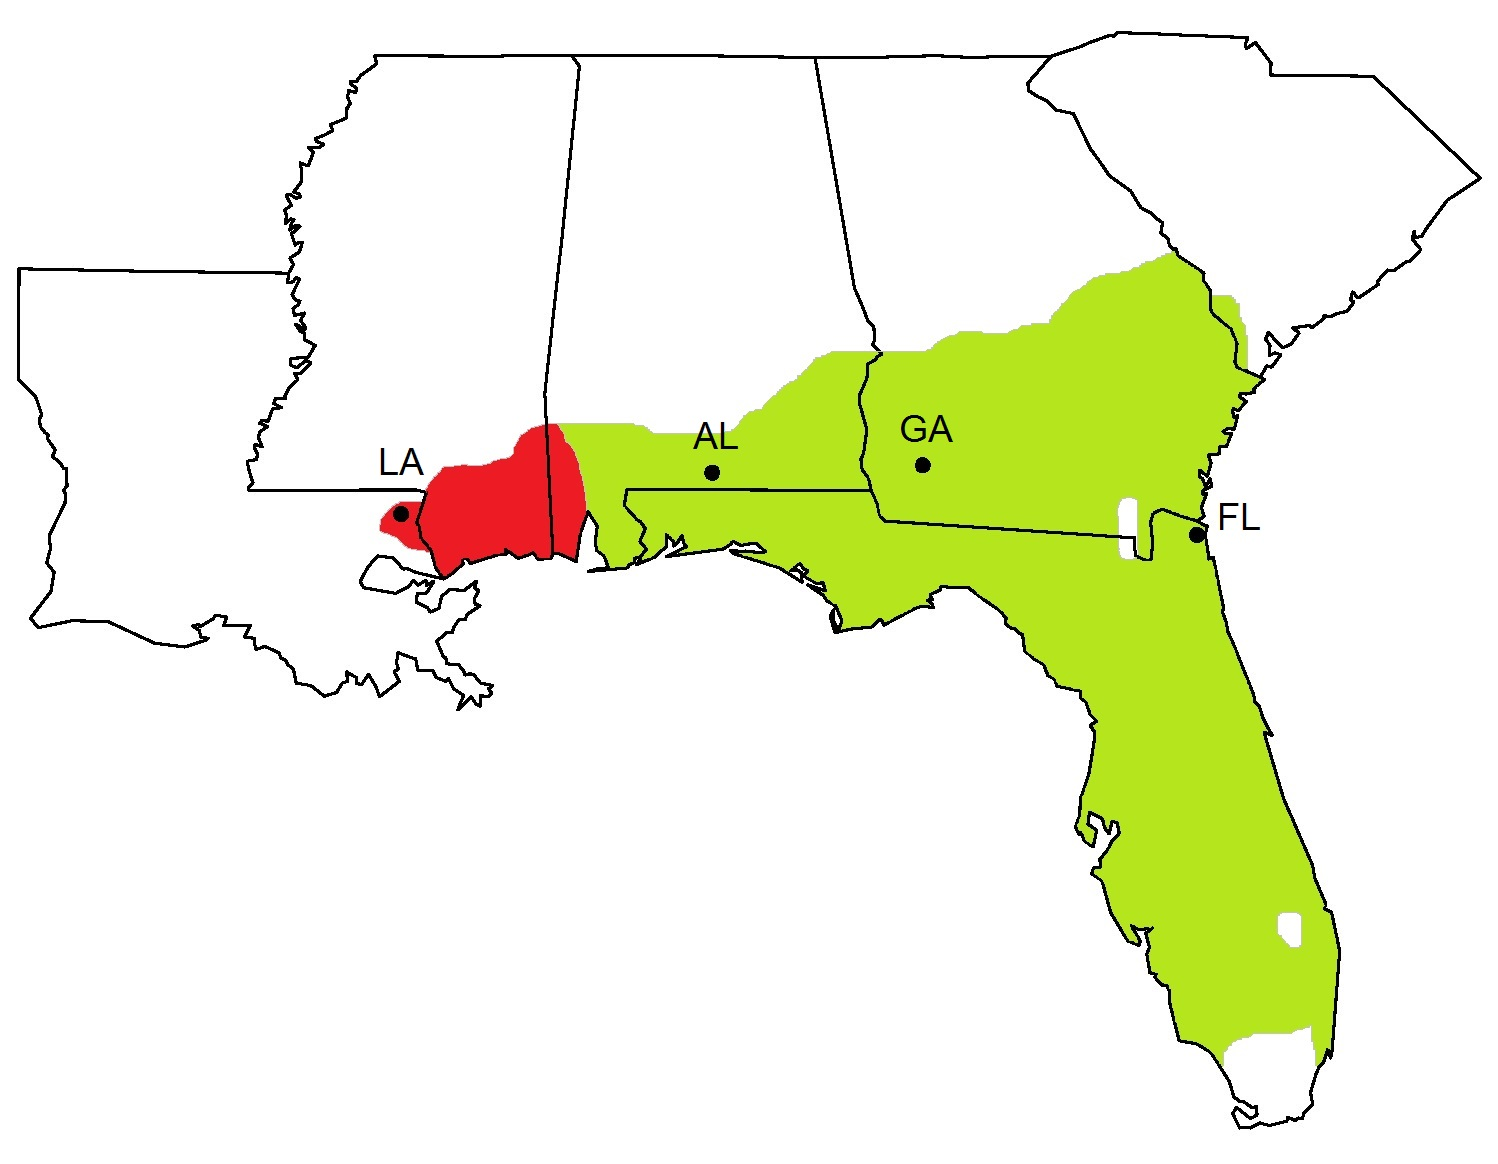
\includegraphics [scale=1.0]{range_map}
\noindent
\textbf{Fig. 1} \textit{Gopherus polyphemus} range map and sampling sites used in this study. Range of western \textit{G. polyphemus} populations darkly shaded on the left with eastern populations lightly shaded on the right. LA for Florida Gas Pipeline, Washington Parish, Louisiana, USA (latitude, longitude, sample size for full microsatellite dataset = 30.78, -90.00; \textit{N} = 36). AL for Solon Dixon, Andalusia, Alabama, USA (31.16, -86.70; \textit{N} = 20). GG for Jones Ecological Research Center, Georgia, USA. (31.23, -84.47; \textit{N} = 26). FL for Private Site, Nassau County, Florida, USA (30.59, -81.56; \textit{N} = 19).\\

\pagebreak{}
\noindent
\begin{knitrout}
\definecolor{shadecolor}{rgb}{0.969, 0.969, 0.969}\color{fgcolor}
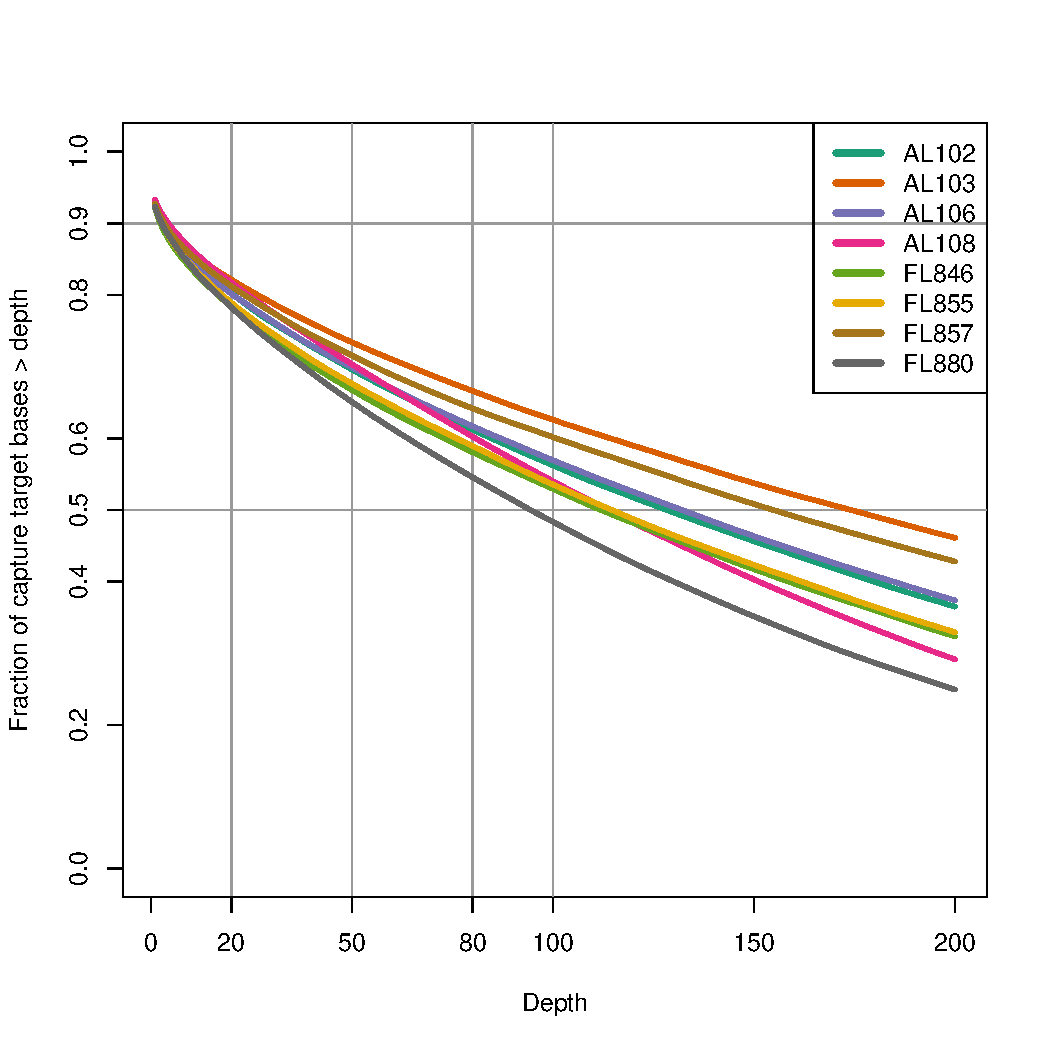
\includegraphics[width=\maxwidth]{figure/Figure-2-1} 

\end{knitrout}
\noindent
\textbf{Fig. 2} Correlations between 10 microsatellites and 17,901 immune gene SNPs for \textit{Gopherus polyphemus} samples. Left column for full microsatellite dataset (101 \textit{G. polyphemus} genotyped at 10 microsatellites) for (A) allelic richness, Pearson's r = 0.411, \textit{P} = 0.294; (B) observed heterozygosity, Pearson's r = 0.945, \textit{P} = 0.028; (C) expected heterozygosity, Pearson's r = 0.976, \textit{P} = 0.012; and (D) \textsc{Fst}, Pearson's r = 0.96, \textit{P} = 0.001. Right column for partial microsatellite dataset (16 \textit{G. polyphemus} genotyped at 10 microsatellites) for (E) allelic richness, Pearson's r = 0.992, \textit{P} = 0.004; (F) observed heterozygosity, Pearson's r = 0.63, \textit{P} = 0.185; (G) expected heterozygosity, Pearson's r = 0.924, \textit{P} = 0.038; and (H) \textsc{Fst}, Pearson's r = 0.968, \textit{P} = 0.001. \textsc{Ar} for allelic richness, \textsc{Ho} for observed heterozygosity, \textsc{He} for expected heterozygosity. \\


\pagebreak{}
\noindent
\begin{knitrout}
\definecolor{shadecolor}{rgb}{0.969, 0.969, 0.969}\color{fgcolor}
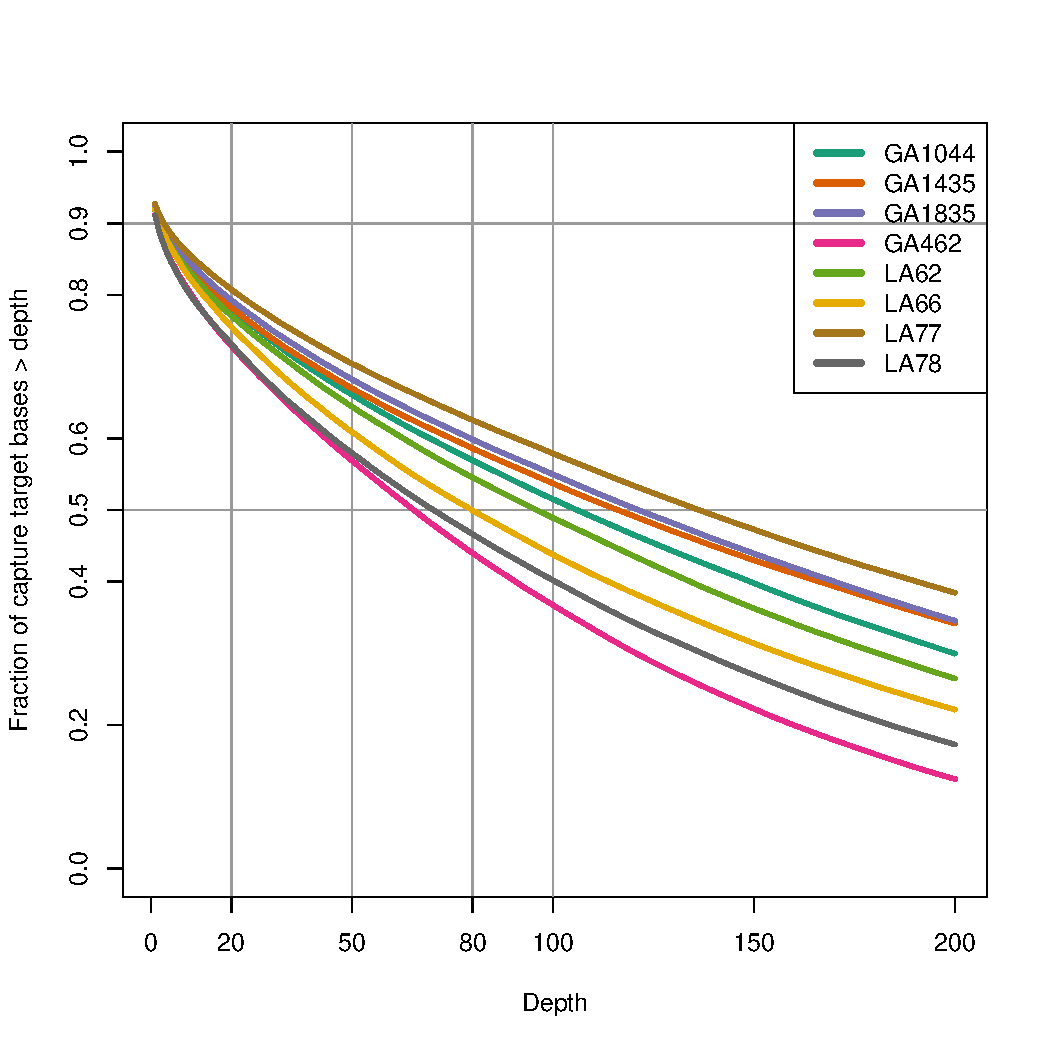
\includegraphics[width=\maxwidth]{figure/Figure-3-1} 

\end{knitrout}
\noindent
\textbf{Fig. 3} Principle component analysis for \textit{Gopherus polyphemus} datasets: (A) the SNP dataset (16 \textit{G. polyphemus} sequenced at 17,901 immune gene SNPs); (B) full microsatellite dataset (101 \textit{G. polyphemus} genotyped at 10 microsatellites); and (C) partial microsatellite dataset (16 \textit{G. polyphemus} genotyped at 10 microsatellites). Circles indicate optimum clusters indentified using \texttt{STRUCTURE} and \texttt{STRUCTURE HARVESTER}.\\

\end{document}
